\documentclass[a4paper,11pt]{article}
\usepackage[utf8]{inputenc}
\usepackage[T1]{fontenc}
\usepackage{lmodern}
\usepackage{subcaption}
\usepackage[siunitx]{circuitikz}
\usepackage{longtable}
\usepackage{titlesec}
\usepackage{graphicx}
\usepackage{amsmath}
\usepackage{multicol}
\usepackage{float}
\usepackage[left=1.5cm, right=3cm, top=1.5cm, bottom=1.5cm]{geometry}
\usepackage[justification=centering]{caption}
\usepackage[txtcentered=true, height=40pt, width=70pt]{thumbs}
\DeclareGraphicsExtensions{.png}

\titleformat*{\section}{\sffamily\LARGE\bfseries}
\titleformat*{\subsection}{\sffamily\Large\bfseries}
\titleformat*{\subsubsection}{\sffamily\large\bfseries}

\pagenumbering{arabic}

\newcommand{\fancythumb}[2]{
	\addthumb{#1}{\large\sffamily\textbf{\space\space#1\vspace{5pt}}}{white}{#2}
}

\begin{document}
\section*{MOSFET-Gleichungen}
\fancythumb{MOSFET}{red}
\subsubsection*{Sperrbereich}
\vspace{-15pt}
\begin{figure}[H]
	\begin{subfigure}{0.49\textwidth}
		\[
			I_{Dn/p} = 0
		\]
	\end{subfigure}
	\begin{subfigure}{0.49\textwidth}
		wenn $ U_{GSn}-U_{Tn} \leq 0$ beim n-MOSFET\\
		wenn $ U_{GSp}-U_{Tp} \geq 0$ beim p-MOSFET
	\end{subfigure}
\end{figure}

\subsubsection*{Widerstandsbereich}
\[
	\boxed{ \quad I_{Dn/p} = \pm\beta_{n/p}\left[(U_{GSn/p}-U_{Tn/p}) U_{DSn/p}-\dfrac{U_{DSn/p}^2}{2}\right](1\pm\lambda_{n/p}\ U_{DSn/p}) \quad }
\]
wenn $0<U_{DSn}<U_{GSn}-U_{Tn}$ und $\lambda_n>0$ beim n-MOSFET (+)\\
wenn $U_{GSp}-U_{Tp}<U_{DSp}<0$ und $\lambda_p>0$ beim p-MOSFET (-)

\subsubsection*{Sättigungsbereich}
\[
	\boxed{ \quad I_{Dn/p}=\pm\dfrac{1}{2}\beta_{n/p}\left(U_{GSn/p}-U_{Tn/p}\right)^2\ (1\pm\lambda_{n/p}\ U_{DSn/p}) \quad }
\]
wenn $U_{DSn}\geq U_{GSn}-U_{Tn}>0$ und $\lambda_n>0$ beim n-MOSFET (+)\\
wenn $U_{DSp}\leq U_{GSp}-U_{Tp}<0$ und $\lambda_p>0$ beim p-MOSFET (-)

\subsubsection*{3D-Plot n-Kanal-MOSFET}
\begin{figure}[H]
\begin{subfigure}{0.32\textwidth}
	\begin{center}
		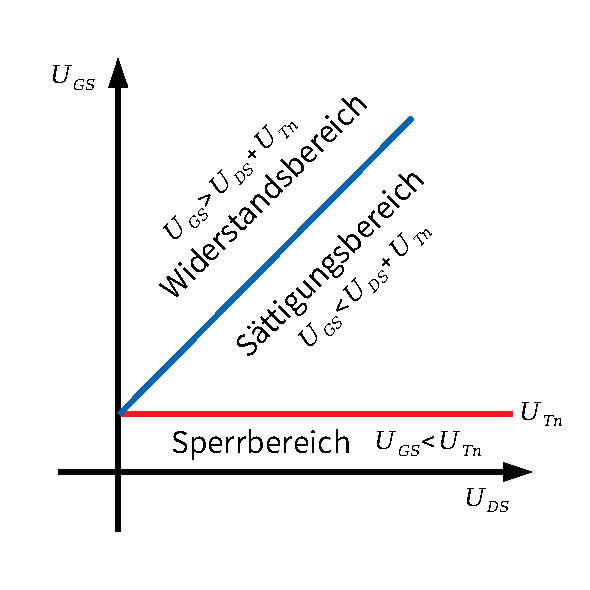
\includegraphics[width=\textwidth]{img/nmosfet_operationmodes.pdf}
	\end{center}
\end{subfigure}
\begin{subfigure}{0.67\textwidth}
	\begin{center}
		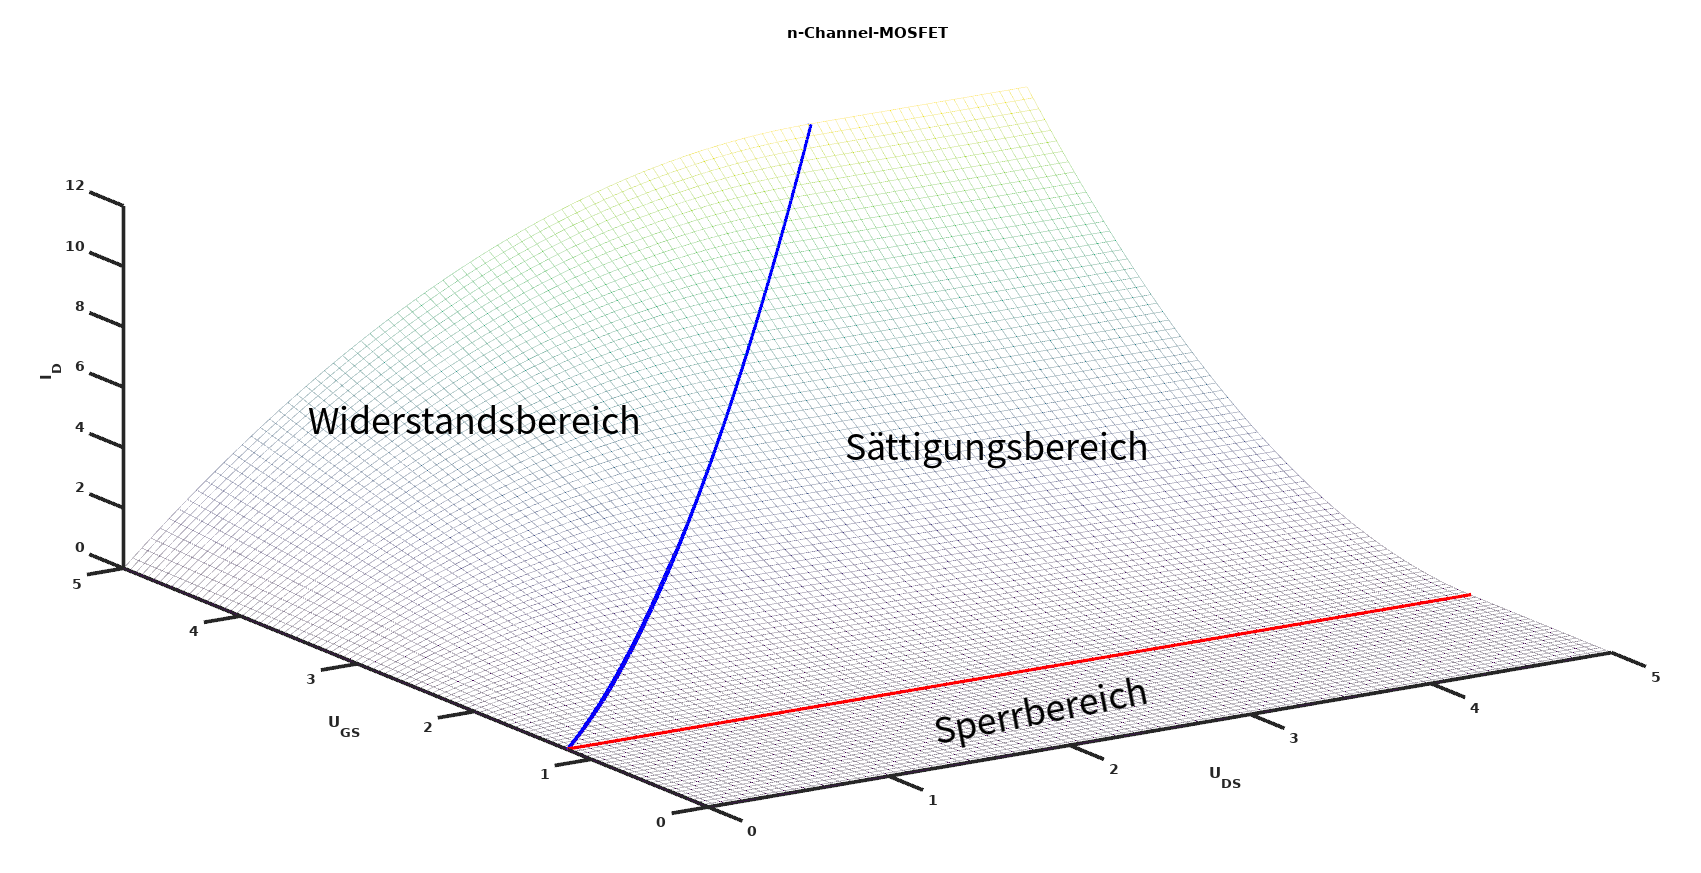
\includegraphics[width=\textwidth]{img/nmosfet_3dplot}
	\end{center}
\end{subfigure}
\end{figure}

\subsubsection*{3D-Plot p-Kanal-MOSFET}
\begin{figure}[H]
\begin{subfigure}{0.32\textwidth}
	\begin{center}
		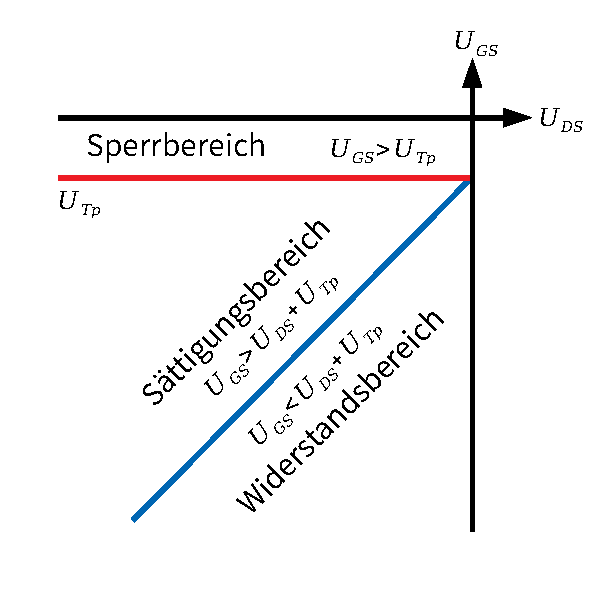
\includegraphics[width=\textwidth]{img/pmosfet_operationmodes.pdf}
	\end{center}
\end{subfigure}
\begin{subfigure}{0.67\textwidth}
	\begin{center}
		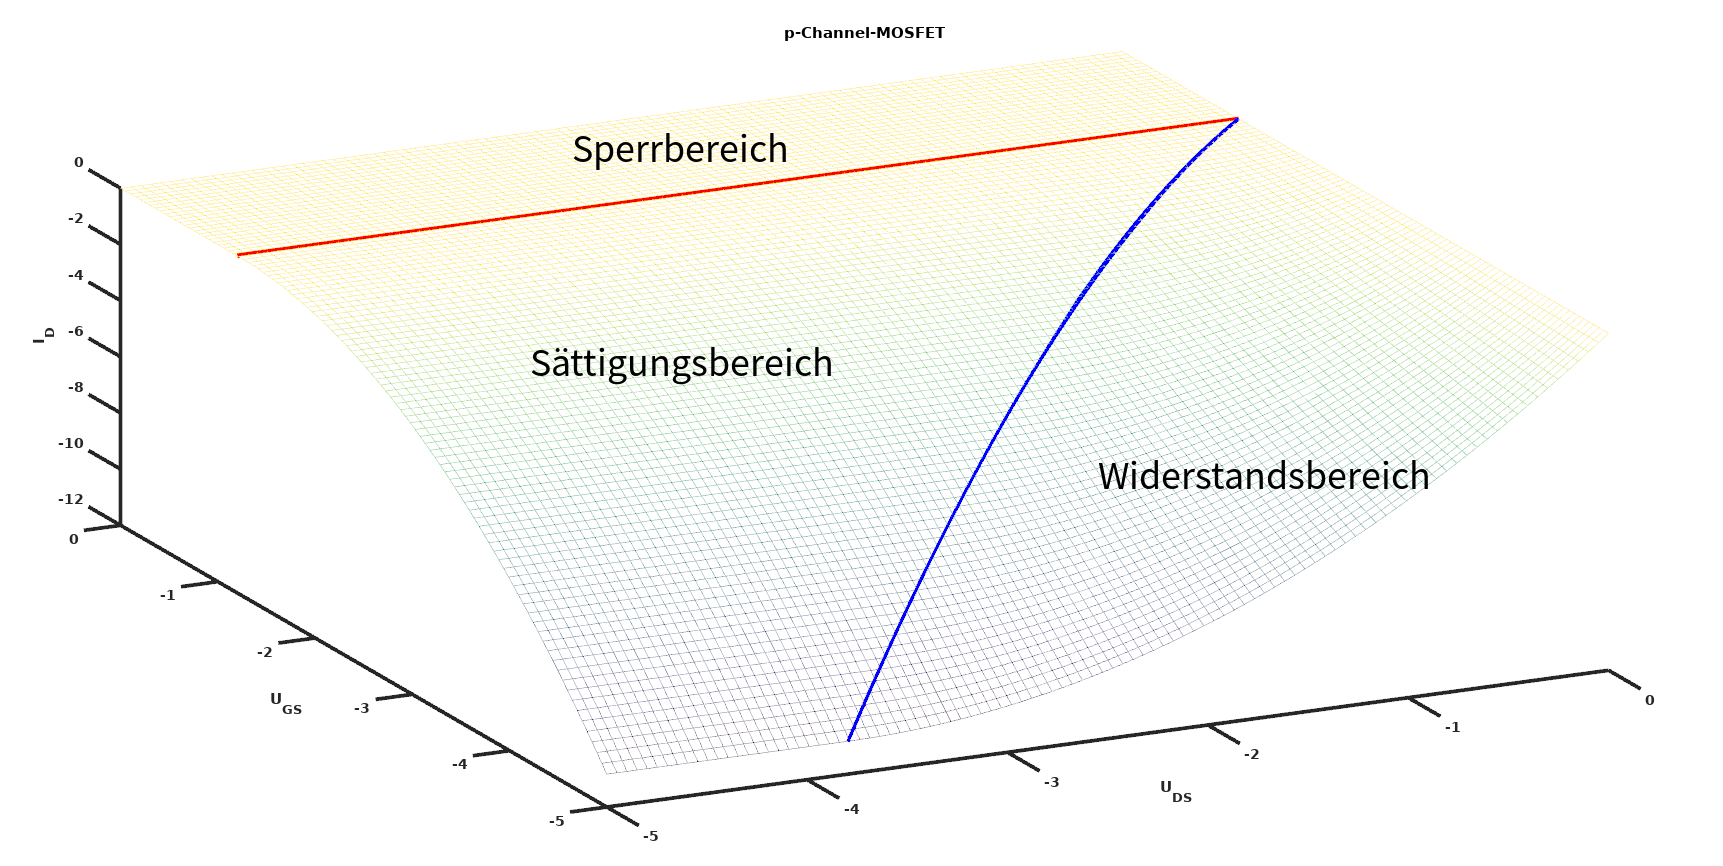
\includegraphics[width=\textwidth]{img/pmosfet_3dplot}
	\end{center}
\end{subfigure}
\end{figure}

\newpage

\section*{Prozessparameter}
\fancythumb{$\beta$ / $k$ / $C$}{black}
\subsection*{Prozessverstärkungsfaktor (\textit{transconductance coefficient})}
\[
	\boxed { \quad \beta_n = k_n ~ \frac{W}{L_{eff}} \quad } \qquad \boxed { \quad \beta_p = k_p ~ \frac{W}{L_{eff}} \quad }
\]

\[
	k_n = \mu_n ~ C_{ox}' = \frac{\mu_n ~ \varepsilon_0 ~ \varepsilon_{SiO_2}}{d_{ox}} \stackrel{typ.}{=} 30 \ldots 200 ~ \frac{\mu A}{V^2}
\]

\[
	k_p = \mu_p ~ C_{ox}' = \frac{\mu_p ~ \varepsilon_0 ~ \varepsilon_{SiO_2}}{d_{ox}} \stackrel{typ.}{=} 15 \ldots 100 ~ \frac{\mu A}{V^2}
\]

\section*{Parasitäre Kapazitäten}
Mit $C_G = C_{ox}' ~ W ~ L$:

\begin{center}
\begin{tabular}{r l}
	$C_{GS} = C_G$ & Gate-Source-Kapazität \\
	$C_j = \frac{2}{3} ~ C_G$ & Drain/Source-Bulk-Sperrschichtkapazität (junction) \\
	$C_{GD} = \frac{2}{3} ~ C_G$ & Gate-Drain-Kapazität
\end{tabular}
\end{center}

\section*{Störabstände (\textit{noise margins})}
\fancythumb{$\text{NM}_{L/H}$}{blue}
\begin{figure}[H]
\begin{center}
	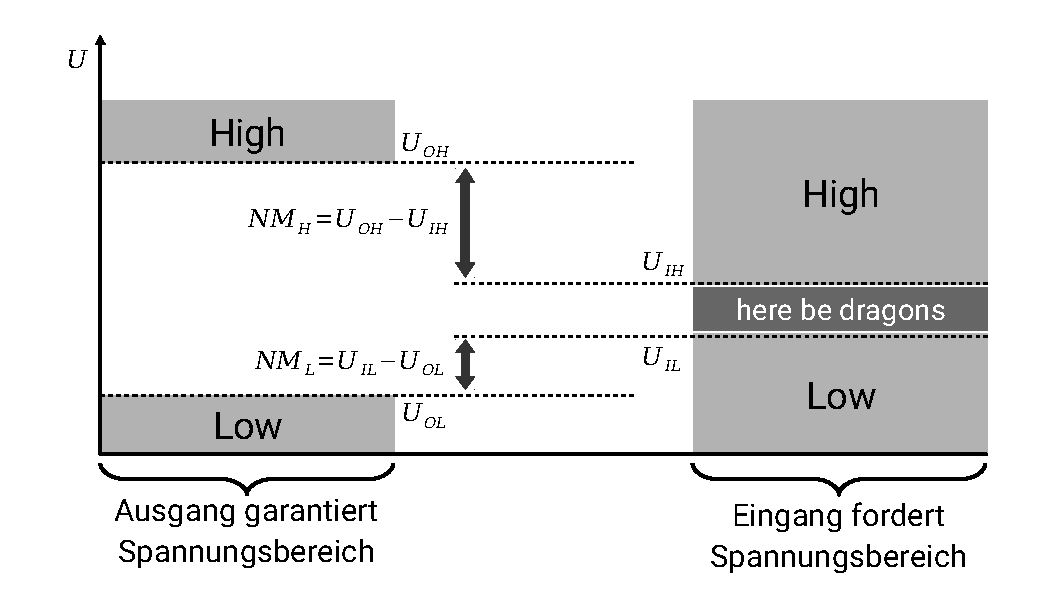
\includegraphics[width=0.9\textwidth]{img/noisemargin.pdf}
\end{center}
\end{figure}

Für symmetrische Dimensionierung $\frac{\beta_n}{\beta_p} = 1$ gilt:
\[
	U_{IL} = \frac{3 ~ U_{DD} - 3 ~ |U_{Tp}| + 5 ~ U_{Tn}}{8} \quad \implies \quad NM_L \approx U_{IL} ~~ \text{für} ~~ U_{OL} \approx 0
\]
\[
	U_{IH} = \frac{5 ~ U_{DD} - 5 ~ |U_{Tp}| + 3 ~ U_{Tn}}{8} \quad \implies \quad NM_H \approx U_{DD} - U_{IH} ~~ \text{für} ~~ U_{OH} \approx U_{DD}
\]

\newpage

\section*{Verzögerungszeiten}
\fancythumb{$t_p$ / $t_{LH}$}{teal}
\subsection*{Laden / Entladen einer Kapazität}
\[
	i(t) = -C_L ~ \frac{\mathrm du_c(t)}{\mathrm dt}
\]

Problem: Finde $t$, stelle also um:
\[
	\mathrm dt = - \frac{C_L}{i(t)} ~ \mathrm du_c
\]

Wobei $i(t)$ durch die Gleichung des entsprechendes MOSFETs bestimmt wird, d.h. nur von $u_c$ abhängt. Die Gesamtzeit ergibt sich dann durch Integration:
\[
	t_{charge} = \pm \int_{U_{\text{start}}}^{U_{\text{end}}} \frac{C_L}{i(u_c)} ~ \mathrm du_c
\]

Mit ``+'' \ldots laden, ``-'' \ldots entladen und Pfeilung so, dass $i > 0$. Als Endwert sollte nicht die vollständige Umladung (also z.B. $U_{DD}$ oder $0V$) verwendet werden, da dieser Wert mathematisch nie erreicht wird.

Häufig auftretende Integrale:
\[
	\int_{U_{\text{start}}}^{U_{\text{end}}} \frac{1}{(a - u)^2} ~ \mathrm du = \left[ \frac{1}{a - u} \right]_{U_{\text{start}}}^{U_{\text{end}}}
\]

\[
	\int_{U_{\text{start}}}^{U_{\text{end}}} \frac{1}{b ~ u - u^2 / 2} ~ \mathrm du = \left[ \frac{1}{b} ~ \ln \left( \frac{u}{u - 2b} \right) \right]_{U_{\text{start}}}^{U_{\text{end}}}
\]

\subsubsection*{Kapazität über NMOS entladen}

\begin{figure}[H]
\centering
\begin{subfigure}{.35\textwidth}
	\centering
	\begin{circuitikz}[european, scale=0.7]
		\draw
			(0,0) node[nigfetebulk](nmos1){}
			(nmos1.S) to node[ground]{} (0, -1)
			(nmos1.D) to ++(0, 0.5) to [short,i<=$i(t)$] ++(1.5, 0) to [C,l^=$C_L$] (1.5, -1) to node[ground]{} (1.5, -1)
			(nmos1.G) to [short, -o] ++(-1.5, 0) node[label={[font=\footnotesize]above:$U_G(t) = U_{DD}$}]{}
		;
	\end{circuitikz}
\end{subfigure}
\begin{subfigure}{.49\textwidth}
	\begin{tabular}{r l}
		\textbf{Startspannung} & $U_{start} = U_{DD}$ \\
		\textbf{Zielspannung} & $U_{end} = 0.1 ~ U_{DD}$ \\
		\textbf{Threshold-Spannung} & $U_{Tn} = 0.2 ~ U_{DD}$ \\
		\textbf{Kanallängenmodulation} & vernachlässigt, $\lambda = 0$
	\end{tabular}
\end{subfigure}
\end{figure}

Abfallzeit:
\[
	\boxed{ \quad t_{HL} \approx 4 ~ \frac{C_L}{\beta_n ~ U_{DD}} \quad }
\]

\subsubsection*{Kapazität über PMOS laden}

\begin{figure}[H]
\centering
\begin{subfigure}{.35\textwidth}
	\centering
	\begin{circuitikz}[european, scale=0.7]
		\draw
			(0,0) node[pigfetebulk, rotate=90](pmos1){}
			(pmos1.G) to [short] ++(0, -1) node[ground,label={[font=\footnotesize]left:$U_G(t) = 0V$}]{}
			(pmos1.S) to [short, -o] ++(-1, 0) node[label={[font=\footnotesize]above:$U_{DD}$}]{}
			(pmos1.D) to [short,i>=$i(t)$] ++(1, 0) to [C,l^=$C_L$] ++(0,-2.4) node[ground]{}
		;
	\end{circuitikz}
	\caption*{Beachte: $i(t) < 0$}
\end{subfigure}
\begin{subfigure}{.49\textwidth}
	\begin{tabular}{r l}
		\textbf{Startspannung} & $U_{start} = 0V$ \\
		\textbf{Zielspannung} & $U_{end} = 0.9 ~ U_{DD}$ \\
		\textbf{Threshold-Spannung} & $U_{Tp} = -0.2 ~ U_{DD}$ \\
		\textbf{Kanallängenmodulation} & vernachlässigt, $\lambda = 0$
	\end{tabular}
\end{subfigure}
\end{figure}

Anstiegszeit:
\[
	\boxed{ \quad t_{LH} \approx 4 ~ \frac{C_L}{\beta_p ~ U_{DD}} \quad }
\]

\subsubsection*{Kapazität über NMOS laden}

\begin{figure}[H]
\centering
\begin{subfigure}{.35\textwidth}
	\centering
	\begin{circuitikz}[european, scale=0.7]
		\draw
			(0,0) node[nigfetebulk, rotate=90](nmos1){}
			(nmos1.G) to [short,-o] ++(-2.5, 0) node[label={[font=\footnotesize]above:$U_G(t) = U_{DD}$}]{}
			(nmos1.D) to [short, -o] ++(-1, 0) node[label={[font=\footnotesize]above:$U_{DD}$}]{}
			(nmos1.S) to [short,i>=$i(t)$] ++(1, 0) to [C,l^=$C_L$] ++(0,-2.4) node[ground]{}
		;
	\end{circuitikz}
	\caption*{Beachte: $i(t) < 0$}
\end{subfigure}
\begin{subfigure}{.49\textwidth}
	\begin{tabular}{r l}
		\textbf{Startspannung} & $U_{start} = 0V$ \\
		\textbf{Zielspannung} & $U_{end} = 0.9 ~ (U_{DD} - U_{Tn})$ \\
		\textbf{Threshold-Spannung} & egal (immer Sättigung) \\
		\textbf{Kanallängenmodulation} & vernachlässigt, $\lambda = 0$
	\end{tabular}
\end{subfigure}
\end{figure}

Anstiegszeit:
\[
	\boxed{ \quad t_{LH} \approx 18 ~ \frac{C_L}{\beta_n ~ (U_{DD} - U_{Tn})} \quad }
\]

\subsubsection*{Über NMOS geladene Kapazität wieder mit NMOS entladen}

\begin{figure}[H]
\centering
\begin{subfigure}{.35\textwidth}
	\centering
	\begin{circuitikz}[european, scale=0.7]
		\draw
			(0,0) node[nigfetebulk](nmos1){}
			(nmos1.S) to node[ground]{} (0, -1)
			(nmos1.D) to ++(0, 0.5) to [short,i<=$i(t)$] ++(1.5, 0) to [C,l^=$C_L$] (1.5, -1) to node[ground]{} (1.5, -1)
			(nmos1.G) to [short, -o] ++(-1.5, 0) node[label={[font=\footnotesize]above:$U_G(t) = U_{DD}$}]{}
		;
	\end{circuitikz}
\end{subfigure}
\begin{subfigure}{.49\textwidth}
	\begin{tabular}{r l}
		\textbf{Startspannung} & $U_{start} = U_{DD} - U_{Tn}$ (\textbf{!!!}) \\
		\textbf{Zielspannung} & $U_{end} = 0.1 ~ (U_{DD} - U_{Tn})$ \\
		\textbf{Threshold-Spannung} & egal (immer linearer Bereich) \\
		\textbf{Kanallängenmodulation} & vernachlässigt, $\lambda = 0$
	\end{tabular}
\end{subfigure}
\end{figure}

Abfallzeit:
\[
	\boxed{ \quad t_{HL} \approx 3 ~ \frac{C_L}{\beta_n ~ (U_{DD} - U_{Tn})} \quad }
\]

\subsection*{Durchschnittliche Verzögerungszeit $t_p$}
Die Durchschnittliche Verzögerungszeit $t_p$ gibt die durchschnittliche Zeit an, die verstreicht zwischen dem Moment, an dem das Eingangssignal den Schaltpunkt $50 \% ~ U_{DD}$ erreicht und dem Moment, an dem das Ausgangssignal ebenfalls den Schaltpunkt überstreicht. Es wird zwischen Anstiegs- und Abfallzeit gemittelt, $t_p = \frac{t_{pHL} + t_{pLH}}{2}$.

Sei Eingangssignal ideal (rechteckförmig) und Umladung erfolgt linear. Dann ist $50 \% ~ U_{DD}$ schon nach der Hälfte der Anstiegs- / Abfallzeit erreicht, d.h. $t_{pHL} = \frac{1}{2} ~ t_{HL}$, $t_{pLH} = \frac{1}{2} ~ t_{LH}$. Somit:
\[
	t_p = \frac{t_{HL} + t_{LH}}{4}
\]

Für den \textbf{CMOS-Inverter} oder Schaltungen mit äquivalenten Transistoren gilt bei symmetrischer Dimensionierung ($\beta_p = \beta_n$): Die Flanken sind symmetrisch und die Verzögerungszeit ist
\[
	\boxed{ \quad t_p \approx \frac{2 ~ C_L}{\beta_n ~ U_{DD}} \quad }
\]

\subsection*{Entladung durch Leckstrom}
Für konstanten Leckstrom $I_{\text{leck}}$ entlädt sich $C$ von $U_{\text{start}}$ auf $U_{\text{end}}$ in
\[
	\boxed { \quad t_{\text{dis}} = C_L ~ \frac{U_{\text{start}} - U_{\text{end}}}{I_{\text{leck}}} \quad }
\]

\newpage

\section*{Dimensionierung und Gateweiten}
\fancythumb{Dimens.}{brown}
\subsection*{Effektive Gateweite bestimmen}
\begin{itemize}
	\item Bestimmen, welche FETs im gegebenen Fall (z.B. Worst-Case) leiten
	\item Nicht leitende FETs erhalten Gateweite 0, andere erhalten physikalische Gateweite
	\item Mit Gateweiten (nächerungsweise) wie mit Leitwerten rechnen und Schrittweise zusammenfassen
	\[
		\boxed{\quad \mathrm{Parallelschaltung:} \quad W_{\parallel} = W_1 + W_2 + \ldots \qquad \mathrm{Reihenschaltung:} \quad W_{ges} = \frac{1}{\frac{1}{W_1} + \frac{1}{W_2} + \frac{1}{\ldots}} \quad}
	\]
	\item Effektive Gateweite ist Ergebnis für die gesamte betrachete Schaltung (z.B. n-Kanal-Zweig)
\end{itemize}

\subsection*{Dimensionierung auf symmetrische Schaltflanken im Worst-Case}
\begin{itemize}
\item Effektive Gateweite des Zweiges bestimmen, für symmetrische Schaltflanken muss gelten
\[
\boxed{\quad W_{P, \mathrm{eff}} \overset{!}{=} \beta_R ~ W_{N, \mathrm{eff}} \overset{\mathrm{typ}.}{=} 2 ~ W_{N, \mathrm{eff}} \quad}
\]
\item Längste MOSFET-Kette im zu dimensionierenden Kanalzweig mit Länge $N$ erhält
\[
	W_1 = W_2 = \ldots = W_N = N ~ W_{\mathrm{eff}}
\]
\item Parallele Kettenschaltungen auf gleiche effektive Gateweite dimensionieren
\end{itemize}

\subsection*{Schaltschwelle des CMOS-Inverters}
\[
	\boxed{ \quad U_e = \frac{U_{DD} + \sqrt{\beta_n / \beta_p} ~ U_{Tn} - |U_{Tp}|}{1 + \sqrt{\beta_n / \beta_p}} \quad }
\]

\newpage
\section*{Verlustleistung}
\fancythumb{Leistung}{violet}
Allgemein setzt sich die Verlustleistung einer \textit{CMOS-Schaltung} aus drei Teilleistungen zusammen:
\begin{itemize}
\item $P_{stat}$: Statische Verlustleistung, wenn dauerhaft über Transistoren ein Strom fließt
\item $P_{dynC}$: Dynamische Verlustleistung zum Laden der Gate-Kapazitäten
\item $P_{dynQ}$: Dynamischen Verlustleistung durch Querstrom, der beim Umschalten eines Inverters fließt, während beide Transistoren leiten
\end{itemize}
\[ \boxed{P=P_{stat}+P_{dynC}+P_{dynQ}} \]

\raggedright
Bei CMOS beläuft sich die statische Verlustleistung $P_{stat}$ im wesentlichen auf die Drain-Leckstöme $I_{Si}\approx10^{-10}A$
\[ \boxed{P_{stat}=U_{DD}\sum_n I_{Si,n}} \]
Die dynamische Verlustleistung, die durch die Lade- und Entladevorgänge abgegeben wird, berechnet sich durch $P_{dynC}=\frac{1}{T}\displaystyle\int_T u(t) ~ i(t) ~ \mathrm{d}t$.\\
Für den Umschaltvorgang von $0$ auf $U_{DD}$ und zurück bei der Frequenz $f_C=1/T$ und der Schaltwahrscheinlichkeit $p$ gilt:
\[ \boxed{P_{dynC}=p\ f_C\ C_L \ U_{DD}^2} \]
Beim Umschalten leiten alle Transistoren kurz, woraus ein dynamischer Querstrom von max. $I_{DQ}\approx\frac{\beta_n}{2}\left(\frac{U_{DD}}{2}-U_{Tn}\right)^2$ folgt. Worst-Case-Abschätzung:
\begin{itemize}
\item Im Mittel fließt halber max. dynamischer Querstrom während Umschaltzeit: $I = I_{DQ} / 2$
\item $t_{LH} = t_{HL}$, \textit{immer} 2 Umschaltvorgänge pro Taktperiode $T$ (z.B. Taktverteilnetzwerk)
\end{itemize}
\[ P_{dynQ} = U_{DD} ~ I ~ \frac{t_{HL} + t_{LH}}{T} = U_{DD} ~ I_{DQ} ~ \frac{t_{HL}}{T} \] 

\subsection*{Power-Delay-Product}
\begin{multicols}{3}
\centering
	Power-Delay-Product: \[ \boxed{W_{PDP}=P\cdot t_p} \]
	Energy-Delay-Product: \[ \boxed{W_{EDP}=P\cdot t_p^2} \]
	Power-Energy-Product: \[ \boxed{W_{PEP}=P^2\cdot t_p} \]
\end{multicols}

\newpage
\section*{Schmitt-Trigger}
\fancythumb{Schmitt}{orange}
\begin{figure}[H]
\centering
\begin{subfigure}{0.44\textwidth}
	\scalebox{0.8}{\begin{circuitikz}[european, scale=0.7]
		% inverter FETs
		\draw
			(0, 0) node[pigfetebulk, label={right:$P_1$}](pmos1){}
			(0,-3) node[pigfetebulk, label={right:$P_2$}](pmos2){}
			(0,-6) node[nigfetebulk, label={right:$N_2$}](nmos2){}
			(0,-9) node[nigfetebulk, label={right:$N_1$}](nmos1){};
		
		\node (uddrail) at ($(pmos1.S) + (0,  0.5)$) {};
		\node (gndrail) at ($(nmos1.S) + (0, -0.5)$) {};

		% inverter interconnects
		\draw
			(uddrail) to [short] (pmos1.S)
			(pmos1.D) to [short] (pmos2.S)
			(pmos2.D) to [short] (nmos2.D)
			(nmos2.S) to [short] (nmos1.D)
			(nmos1.S) to [short] (gndrail) node[ground]{};

		% input interconnects
		\draw
			(pmos1.G) to [short, -*]
			(pmos2.G) to [short, -*]
			(nmos2.G) to [short]
			(nmos1.G);

		% input terminal
		\draw
			($0.5*(pmos2.G)+0.5*(nmos2.G)$) to [short, *-o] ++(-1,0)
			node[label={[font=\small]left:$U_e$}] {};

		\node (center) at ($0.5*(pmos2.D)+0.5*(nmos2.D)$) {};

		% output + output terminal
		\node (output) at ($(center)+(8,0)$) {};
		\draw
			(center) to [short, *-o]
			(output) node[label={[font=\small]right:$U_a$}] {};

		% N_3 NMOS
		\draw
			($0.5*(nmos1.D)+0.5*(nmos2.S)+(3,0)$) node[nigfetebulk, rotate=-90, label={below:$N_3$}](nmos3){}
			($0.5*(nmos1.D)+0.5*(nmos2.S)$) [short, *-] to (nmos3.S)
			(nmos3.G |- center) [short, *-] to (nmos3.G);

		\draw ($0.5*(nmos1.D)+0.5*(nmos2.S)+(1.5,0.1)$) node[label={[font=\small]below:$U_X$}] {};

		\node (n3drain) at ($(nmos3.D) + (1,0)$) {};
		\draw
			(nmos3.D) [short] to
			(n3drain) to [short, -*] (uddrail -| n3drain);

		% P_3 PMOS
		\draw
			($0.5*(pmos1.D)+0.5*(pmos2.S)+(3,0)$) node[pigfetebulk, rotate=90, yscale=-1, label={above:$P_3$}](pmos3){}
			($0.5*(pmos1.D)+0.5*(pmos2.S)$) [short, *-] to (pmos3.D)
			(pmos3.G |- center) [short, *-] to (pmos3.G);

		\draw ($0.5*(pmos1.D)+0.5*(pmos2.S)+(1.5,-0.1)$) node[label={[font=\small]above:$U_Y$}] {};

		\node (p3drain) at ($(pmos3.S) + (2,0)$) {};
		\draw
			(pmos3.S) [short] to
			(p3drain) to [short] (gndrail -| p3drain) node[ground]{};

		% Udd rail
		\draw
			(uddrail) [short] to
			(uddrail -| n3drain) [short, -o] to
			(output |- uddrail) node[label={[font=\small]right:$U_{dd}$}] {};;
	\end{circuitikz}}
\end{subfigure}
\begin{subfigure}{0.54\textwidth}
	\paragraph{Bei steigendem $U_e = 0V \rightarrow U_{DD}$} beginnt $N_1$ beim Überschreiten von $U_e = U_{Tn}$ im Sättigungsbereich zu leiten. $N_3$ leitet ständig an der Grenze zwischen \textit{Sperr}- und Sättigungsbereich ($U_{GSN3} = U_{DSN3} = U_{DD} - U_X$) $\implies$ $U_X$ fällt. Sobald $U_{GSN2} = U_e - U_X > U_{Tn}$ kippt der Schmitt-Trigger. \newline

	\paragraph{Bei fallendem $U_e = U_{DD} \rightarrow 0V$} beginnt $P_1$ beim Unterschreiten von $U_e = U_{DD} + U_{Tp}$ im Sättigungsbereich zu leiten. $P_3$ leitet ständig an der Grenze zwischen \textit{Sperr}- und Sättigungsbereich ($U_{GSP3} = U_{DSP3} = U_{DD} - U_Y$) $\implies$ $U_Y$ steigt. Sobald $U_{GSP2} = U_e - U_Y < U_{Tp}$ kippt der Schmitt-Trigger.
\end{subfigure}
\end{figure}

\subsection*{Schaltschwellen}
Für $\beta_{n/p} = k_{n/p} ~ \frac{W_{n/p}}{L}$ und Näherung $I_{DN2} \approx 0$ bzw. $I_{DP2} \approx 0$ kurz vor dem Schaltzeitpunkt folgt für die obere Schwelle $U_{M+}$ und für die untere Schwelle $U_{M-}$:
\[
	\boxed { \quad U_{M+} = \frac{\sqrt{W_{N3} / W_{N1}} ~ U_{DD} + U_{Tn}}{\sqrt{W_{N3}/W_{N1}} + 1} \quad } \qquad \boxed { \quad U_{M-} = \frac{U_{DD} + U_{Tp}}{\sqrt{W_{P3}/W_{P1}} + 1} \quad }
\]
Obere und untere Schwelle können \textit{unabhängig} voneinander durch Dimensionierung von $N_1$ / $N_3$ bzw. $P_1$ / $P_3$ konfiguriert werden.

\subsubsection*{Ansatz beispielhaft für NMOS}
Schaltung kippt, sobald $N_2$ leitet, d.h. $U_{GSN2} = U_e - U_X > U_{Tn}$, Schaltpunkt also bei $U_X = U_e - U_{Tn}$. Bestimme $U_e$ für Kipppunkt.\\
Ansatz: $I_{DN3} = I_{DN1}$ mit $N_3$ \ldots Sättigung, $N_1$ \ldots Grenze linear / Sättigung, einfacher Sättigung.
\[
	\frac{1}{2} \beta_{N3} ~ (U_{GSN3} - U_{Tn})^2 = \frac{1}{2} \beta_{N1} ~ (U_{GSN1} - U_{Tn})^2
\]
Mit $U_{GSN3} = U_{DD} - U_X$ und $U_{GSN1} = U_e$ folgt:
\[
	\beta_{N3} ~ (U_{DD} - U_X - U_{Tn})^2 =\beta_{N1} ~ (U_e - U_{Tn})^2	
\]
Setze $U_X = U_e - U_{Tn}$ ein:
\[
	\beta_{N3} ~ (U_{DD} - U_e)^2 =\beta_{N1} ~ (U_e - U_{Tn})^2	
\]
\[
	\sqrt{\frac{\beta_{N3}}{\beta_{N1}}} ~ (U_{DD} - U_e) = U_e - U_{Tn}
\]
Umformen nach $U_{M+} = U_e$ führt mit $\beta \sim W$ zur obigen Gleichung.
\end{document}